\documentclass[tikz]{standalone}
\usetikzlibrary{shapes.geometric}    % trapezium
\usetikzlibrary{arrows}              % arrow tips
\usepackage{amsmath}
\usepackage{bm}                      % boldsymbol
\usepackage{makecell}                % makecell
\usetikzlibrary{matrix,calc}

\begin{document}
    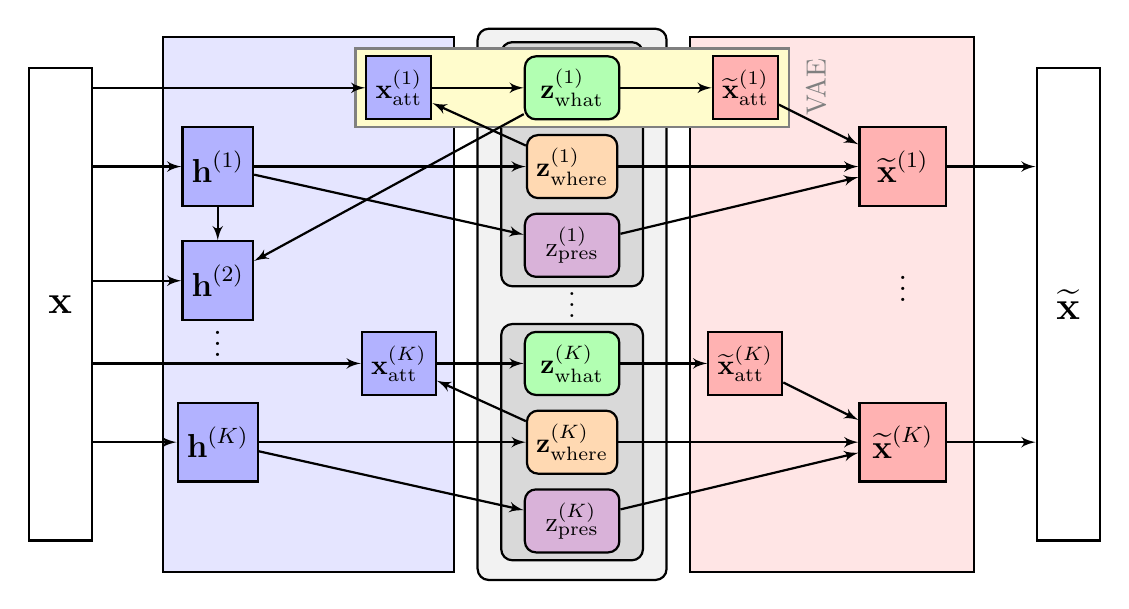
\begin{tikzpicture}[baseline=0, >=latex',thick]
      \node (rect) at (0,0)
      [draw, thick, minimum width=0.8cm, minimum height=6cm, name=x]
      {\Large{$\textbf{x}$}};


      \node (rect) at (3.15, 0)
      [draw, thick, minimum height=6.8cm, minimum width=3.7cm, fill=blue!10] {};

      \node (rect) at (9.8, 0)
      [draw, thick, minimum height=6.8cm, minimum width=3.6cm, fill=red!10] {};

      \node (rect) at (2,1.75)
      [draw, thick, minimum width=0.8cm, minimum height=1cm, name=h1, fill=blue!30]
      {\large{$\textbf{h}^{(1)}$}};

      \node (rect) at (2,0.3)
      [draw, thick, minimum width=0.8cm, minimum height=1cm, name=h2, fill=blue!30]
      {\large{$\textbf{h}^{(2)}$}};


      \node at (2,-0.4) [ minimum width=0.8cm, minimum height=0.3cm, name=hp]
      {\large{$\vdots$}};
      % \node at (2,-0.6) [ minimum width=0.8cm, minimum height=0.3cm, name=hp]
      % {\large{$\vdots$}};

      \node (rect) at (2,-1.75)
      [draw, thick, minimum width=0.8cm, minimum height=1cm, name=hN, fill=blue!30]
      {\large{$\textbf{h}^{(K)}$}};

      \draw [->] (h1) -- (h2);

      \draw [->] ($(x.east) + (0, 1.75)$) -- (h1.west);
      \draw [->] ($(x.east) + (0, 0.3)$) -- (h2.west);
      \draw [->] ($(x.east) + (0, -1.75)$) -- (hN.west);

      \node [rectangle, rounded corners] at (6.5, 0)
      [draw, thick, minimum width=2.4cm, minimum height=7cm, name=z, fill=gray!10]
      {};


      % \node (rect) at (6.5, 2.75)
      % [draw=gray, thick, minimum width=5.5cm, minimum height=1.0cm, name=VAE,
      % fill=yellow!20,
      % label={[xshift=3.1cm, yshift=-1.cm]\rotatebox{90}{\textcolor{gray}{VAE}}}]
      % {};

      \node [rectangle, rounded corners] at (6.5, 1.78)
      [draw, thick, minimum width=1.8cm, minimum height=3.1cm, name=z1, fill=gray!30]
      {};

      % yellow box in foreground
      \node (rect) at (6.5, 2.75)
      [draw=gray, thick, minimum width=5.5cm, minimum height=1.0cm, name=VAE,
      fill=yellow!20,
      label={[xshift=3.1cm, yshift=-1.cm]\rotatebox{90}{\textcolor{gray}{VAE}}}]
      {};

      \node (rect) at (4.3,2.75)
      [draw, thick, minimum width=0.8cm, minimum height=0.8cm, name=xatt1, fill=blue!30]
      {{$\textbf{x}_{\text{att}}^{(1)}$}};
      \node (rect) at (8.7,2.75)
      [draw, thick, minimum width=0.8cm, minimum height=0.8cm, name=xatt1t, fill=red!30]
      {{$\widetilde{\textbf{x}}_{\text{att}}^{(1)}$}};

      \node [rectangle, rounded corners] at (6.5,2.75)
      [draw, thick, minimum width=1.2cm, minimum height=0.8cm, name=z1what, fill=green!30]
      {{$\textbf{z}_{\text{what}}^{(1)}$}};

      \node [rectangle, rounded corners] at (6.5,1.75)
      [draw, thick, minimum width=0.8cm, minimum height=0.8cm, name=z1where, fill=orange!30]
      {{$\textbf{z}_{\text{where}}^{(1)}$}};

      \node [rectangle, rounded corners] at (6.5,0.75)
      [draw, thick, minimum width=1.2cm, minimum height=0.8cm, name=z1pres, fill=violet!30]
      {{$\text{z}_{\text{pres}}^{(1)}$}};

      \node (rect) at (6.5,0.1)
      [minimum width=1.2cm, minimum height=0.8cm, name=dots] {{$\vdots$}};

      \node (rect) at (4.3,-0.75)
      [draw, thick, minimum width=0.8cm, minimum height=0.8cm, name=xattN, fill=blue!30]
      {{$\textbf{x}_{\text{att}}^{(K)}$}};

      \node (rect) at (8.7,-0.75) [draw, thick, minimum width=0.8cm, minimum height=0.8cm,
      name=xattNt, fill=red!30] {{$\widetilde{\textbf{x}}_{\text{att}}^{(K)}$}};

      \node [rectangle, rounded corners] at (6.5, -1.75)
      [draw, thick, minimum width=1.8cm, minimum height=3cm, name=zN, fill=gray!30]
      {};


      \node [rectangle, rounded corners] at (6.5,-0.75)
      [draw, thick, minimum width=1.2cm, minimum height=0.8cm, name=zNwhat, fill=green!30]
      {{$\textbf{z}_{\text{what}}^{(K)}$}};

      \node [rectangle, rounded corners] at (6.5,-1.75)
      [draw, thick, minimum width=0.8cm, minimum height=0.8cm, name=zNwhere, fill=orange!30]
      {{$\textbf{z}_{\text{where}}^{(K)}$}};

      \node [rectangle, rounded corners] at (6.5,-2.75)
      [draw, thick, minimum width=1.2cm, minimum height=0.8cm, name=zNpres, fill=violet!30]
      {{$\text{z}_{\text{pres}}^{(K)}$}};

      % \draw [->] (h1) -- (xatt1);
      \draw [->] ($(x.east) + (0, 2.75)$) -- (xatt1.west);
      \draw [->] (h1) -- (z1where);
      \draw [->] (h1) -- (z1pres);
      \draw [->] (z1what) -- (h2);
      \draw [->] (z1where) -- (xatt1);
      \draw [->] (xatt1) -- (z1what);
      \draw [->] (z1what) -- (xatt1t);

      % \draw [->] (hN) -- (xattN);
      \draw [->] ($(x.east) + (0, -0.75)$) -- (xattN.west);
      \draw [->] (hN) -- (zNwhere);
      \draw [->] (hN) -- (zNpres);
      \draw [->] (zNwhere) -- (xattN);
      \draw [->] (xattN) -- (zNwhat);
      \draw [->] (zNwhat) -- (xattNt);

      \node (rect) at (10.7, 1.75)
      [draw, thick, minimum width=1.1cm, minimum height=1cm, name=x1t, fill=red!30]
      {\large{$\widetilde{\textbf{x}}^{(1)}$}};

      \node (rect) at (10.7,0.3)
      [minimum width=0.8cm, minimum height=1cm] {\large{$\vdots$}};

      \node (rect) at (10.7,-1.75)
      [draw, thick, minimum width=1.1cm, minimum height=1cm, name=xNt, fill=red!30]
      {\large{$\widetilde{\textbf{x}}^{(K)}$}};

      \draw [->] (xatt1t) -- (x1t);
      \draw [->] (z1where) -- (x1t);
      \draw [->] (xattNt) -- (xNt);
      \draw [->] (z1pres) -- (x1t);
      \draw [->] (zNwhere) -- (xNt);
      \draw [->] (zNpres) -- (xNt);

      \node (rect) at (12.8,0)
      [name=xrec, draw, thick, minimum width=0.8cm, minimum height=6cm]
      {\Large{$\widetilde{\textbf{x}}$}};

      \draw [->] (x1t.east) -- ($(xrec.west) + (0, 1.75)$);
      \draw [->] (xNt.east) -- ($(xrec.west) + (0, -1.75)$);
    \end{tikzpicture}
\end{document}
